% vim: set tw=78 tabstop=4 shiftwidth=4 aw ai:

\chapter{A Novel BitTorrent Tracker Overlay for Swarm Unification}
\label{chapter:unified-tracker}

The role of the BitTorrent tracker, and the problem of it being a single point
of failure, may be circumvented through the use of PXE (\textit{Peer
Exchange}) and DHT (\textit{Distributed Hash Table})~\cite{dht-paper}. These
new technologies are new ways of discovering peers, without having to rely on
the BitTorrent tracker. There needs to be an initial bootstrap phase; control
information is provided from one peer to another peer. Most implementations
nowadays provide PXE or DHT, coupled with the use of a tracker. In many cases,
such as libtorrent-rasterbar, the implementation may simultaneously use both
DHT and the classical tracker data.

The role of extending tracker functionality is to provide redundancy and
generally simplify the architecture. Our goal of building a tracker overlay
for swarm unification aims to enhance swarms, and allow the presence of
multiple peers and seeders in a swarm, with the potential benefit of increased
swarm speed. As the health of a swarm not only relies on the number of peers,
but also on the ratio of seeders versus leechers, approaches such as building
private swarms or providing moderation are important. These approaches provide
the means for extending seeder availability within the swarm and providing
a constant flow of data.

Trackers are server-only entities. They are contacted by peers to update
internal information and provide information to clients. The tracker database
stores information about peers taking part in a swarm and statistical
information about peers, such as download size. This information have been
used heavily by Bardac~et~al.~\cite{tracker-mon} in building a tracker
monitoring service. Our proposal is to enhance existing tracker messages and
allow trackers to interconnect -- that is to communicate with each other, on
top of the existing communication with peers in the swarm.

\section{Context and Objective}
\label{sec:unified-tracker:context}

We address the issue of unifying separate swarms that take
part in a session sharing the same file. We propose a tracker unification
protocol that enables disparate swarms, using different .torrent files, to
converge. We define swarm unification as enabling clients from different
swarms to communicate with each other. The basis for the unification is a
``tracker-centric convergence protocol'' through which trackers form an
overlay network and send peer information to each other.

The goal of the tracker swarm unification protocol is the integration of peers
taking part in different swarms that share the same file. These swarms, named
\textbf{common swarms}, use the same content but different trackers.

We have designed and implemented a tracker network overlay that enables
trackers to share information and integrate peers in their respective swarms.
The overlay is based on the Tracker Swarm Unification Protocol (TSUP) that
allows update notification and delivery to trackers from the overlay. The
protocol design is inspired by routing protocols in computer networks.

The protocol proposed in this article, named \textbf{Tracker Swarm Unification
Protocol (TSUP)}, renders possible the unification of swarms which share
the same files, by employing a tracker network overlay. A tracker which
implements this protocol will be referred here as an \textbf{unified tracker}.

\begin{figure}[h]
  \begin{center}
    \includegraphics[width=0.7\textwidth]{src/img/unified-tracker/unified-trackers}
  \end{center}
  \caption{Unified trackers}
  \label{fig:unified-tracker:unified-trackers}
\end{figure}

Torrent files created for the same content have the same \textit{info_hash}.
As such, in swarms that share the same file(s) (common swarms), peers will announce
to the tracker the same \textit{info_hash}. Therefore, TSUP capable trackers
can ``unify'' them by communicating with each other in order to change
information about peers which contribute to shared files with the same
\textit{info_hash}.  In order to accomplish this, unified trackers send
periodic updates to each other, containing information about the peers from
the network.

\section{Swarm Unification Protocol}
\label{sec:unified-tracker:swarm-unification}

As mentioned above, \textit{TSUP} is the acronym for \textit{Tracker Swarm
Unification Protocol}. TSUP is responsible with the communication between
trackers for peer exchange information in common swarms.

\subsection{Protocol Overview}
\label{subsec:unified-tracker:protocol-overview}

For transport layer communication, the protocol uses UDP (User Datagram
Protocol) to reduce resource consumption. A tracker already possesses a lot of
TCP (Transport Control Protocol) connections with other peers. Adding
more TCP connections to each neighboring tracker would increase TSUP overhead
too much for a big tracker overlay. The messages passed from one tracker to
another do not need TCP's flow control and need a lower level of reliability
than TCP as it will be explained below. The simplicity of the UDP protocol
gives the advantage of a smaller communication overhead.

In TSUP's operation the following processes may be identified:
\begin{itemize}
    \item \textbf{Virtual connections establishment process:} A
    three-way-handshake responsible with establishing a UDP ``connection''
    between two linked trackers at the application layer. The process is
    started by a SYN packet (synchronization packet).
    \item \textbf{Unification process:} The trackers exchange unification
    packets (named \textit{SUMMARY} packets) during a three-way-handshake in
    order to find out which are the common swarms.
    \item \textbf{Updating process:} The trackers exchange peers from common
    swarms, encapsulated in \textit{UPDATE} packets.
    \item \textbf{Election process:} The establishment of a \textit{swarm
    leader} which is responsible with receiving all updates from the
    neighboring linked trackers, aggregating them and sending the results
    back.
\end{itemize}

The \textit{unification process} includes an updating process in its
three-way-handshake, such that the two operations, unification and update, are
run in pipeline. Whenever a new torrent file is registered to the tracker, a
new swarm is created. The unification process is triggered and a SUMMARY
packet is immediately sent to each neighboring tracker, informing the others of the new swarm.

The \textit{updating process} is started periodically, such that UPDATE
packets are sent at a configurable interval of time to each tracker in a
common swarm. A typical update interval is 30 seconds.

In order to maintain the virtual connections between trackers, HELLO packets
are sent periodically, acting as a keep-alive mechanism. A typical HELLO
interval is 10 seconds, but its value may be changed from protocol
configuration. If no HELLO packet is received during a configurable interval,
called disconnect interval, the virtual connection is dropped and the virtual
connection establishment process is restarted for that link by sending a SYN
packet.

\subsection{Tracker Awareness}
\label{subsec:unified-tracker:tracker-awareness}

Tracker communication is conditioned by awareness. For this purpose, in the
current version of the protocol, each tracker is configured statically with a
list of other communicating trackers. Each element of the list represents a
\textit{link} which is identified by the tracker host name (URL or IP address)
and port. Other parameters for the link may be configured; some of them may be
specific to the implementation. If the virtual connection establishment
process is successful, the link becomes a virtual connection, which is
conserved with keep-alive packets (\texttt{HELLO} packets).

\subsection{Tracker Networks}
\label{subsec:unified-tracker:tracker-networks}

To improve TSUP's scalability, trackers may be grouped together in networks
named \textbf{tracker networks}. Connections in all tracker networks are full
mesh. Two networks are connected with the aid of \textbf{border trackers} (see
Figure~\ref{fig:unified-tracker:tracker-networks}).

\begin{figure}[h]
  \begin{center}
    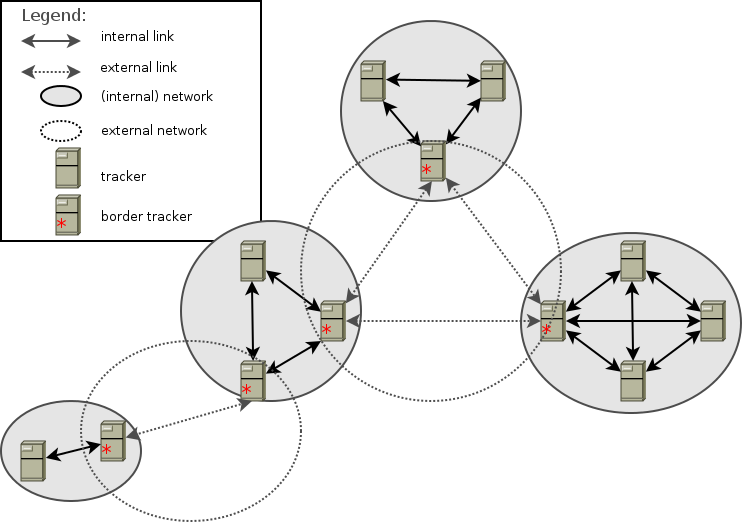
\includegraphics[width=0.7\textwidth]{src/img/unified-tracker/tracker-networks}
  \end{center}
  \caption{Tracker Networks}
  \label{fig:unified-tracker:tracker-networks}
\end{figure}

To configure a topology which contains multiple networks, each link of each
tracker must be set as an \textbf{internal link} or an \textbf{external link}
(see Figure~\ref{fig:unified-tracker:tracker-networks}). Trackers connected
with internal links are part of the same \textit{tracker network}; trackers
connected with external links are part of other networks. However, the ones
from the first category may also be classified as belonging to an
\textbf{internal network} and the ones from the second category as being from
an \textbf{external network}.

A complete graph, using internal links as edges is an \textit{internal
network}, and a complete graph with external links as edges is an
\textit{external network} (see
Figure~\ref{fig:unified-tracker:tracker-networks}). A tracker which has both
internal and external links is a border tracker. Peer information received
from an internal network originates from \textbf{internal peers} while
information received from an external network originates from \textbf{external
peers}. Peers connected to a tracker with TCP, via the BitTorrent protocol,
are called \textbf{own peers}. The links between trackers in a network,
whether internal or external, must be full mesh.

In order to use a scalable and low resource consuming communication within a
network, trackers are organized in groups depending on the unified swarm.
Therefore a tracker may belong to more than one group at the same time, the
number of groups it belongs being equal with the number of swarms present on
that tracker. Each group contains a \textbf{swarm leader} responsible for
sending peer updates to peers in the group. The other group members, instead
of sending updates to other members on a full mesh graph, it sends updates to
the swarm leader on a tree graph, reducing updating overhead. These updates
propagate to other peers in the group.

In accordance to graph theory, the number of updates sent in a swarm without
the swarm leader mechanism (full mesh) is computed by using the formula below:

%\vspace{3mm}

\begin{equation}\label{updates-fullmesh}
UPDATES_{full mesh} = 2\cdot\frac{n(n-1)}{2} = n(n-1)
\end{equation}

%\vspace{3mm}

The number of updates sent within a swarm using the swarm leader mechanism
(tree) are:

%\vspace{3mm}

\begin{equation}\label{updates-swarmleader}
UPDATES_{swarm leader} = 2(n-1)
\end{equation}

%\vspace{3mm}

As may be observed from the formulas above the complexity decreases from
$O(n^{2})$ in a full mesh update scheme to $O(n)$ with the swarm leader
scheme.

Each swarm contains two swarm leaders, one for the internal network (which
sends updates through internal links), called \textit{internal swarm leader}
and one for the external network (which communicates updates through external
links), named \textit{external swarm leader}.

Grouping trackers in networks increases system scalability, but also network
convergence time. The update timers can be set to a lower value for border
trackers to limit convergence overhead.  The system administrator should opt
between scalability and convergence and adapt the protocol parameters to the
specific topology.

\section{Experimental Setup}
\label{sec:unified-tracker:setup}

TSUP testing activities used a virtualized infrastructure and a
Peer-to-Peer testing framework running on top of it. We were able to deploy
scenarios employing various swarms, ranging from a 4-peer and 1-tracker swarm
to a 48-peer and 12-tracker swarm. Apart from testing and evalution, the
infrastructure has been used to compare the proposed tracker overlay network
with classical swarms using a single tracker and the same number of peers. We
will show that a unified swarm has similar performance when compared to a
single tracker (classical) swarm.

In order to deploy a large number of peers we have used a thin virtualization
layer employing OpenVZ\footnote{\url{http://wiki.openvz.org}}. OpenVZ is a
lightweight solution that allows rapid creation of virtual machines (also
called containers). All systems are identical with respect to hardware and
software components. The deployed experiments used a single OpenVZ container
either for each tracker or peer taking part in a swarm. A virtualized network
has been build allowing direct link layer access between systems -- all
systems are part of the same network; this allows easy configuration and
interraction.

The experiments made use of an updated version of hrktorrent, a lightweight
application built on top of libtorrent-rasterbar. Previous
experiments~\cite{bt-vi} have shown libtorrent-rasterbar outperforming other
BitTorrent experiments leading to its usage in the current experiments. The
experiments we conducted used a limitation typical to ADSL2+ connections (24
Mbit download speed limitation, 3 Mbit upload speed limitation).

\begin{figure}[h]
  \begin{center}
    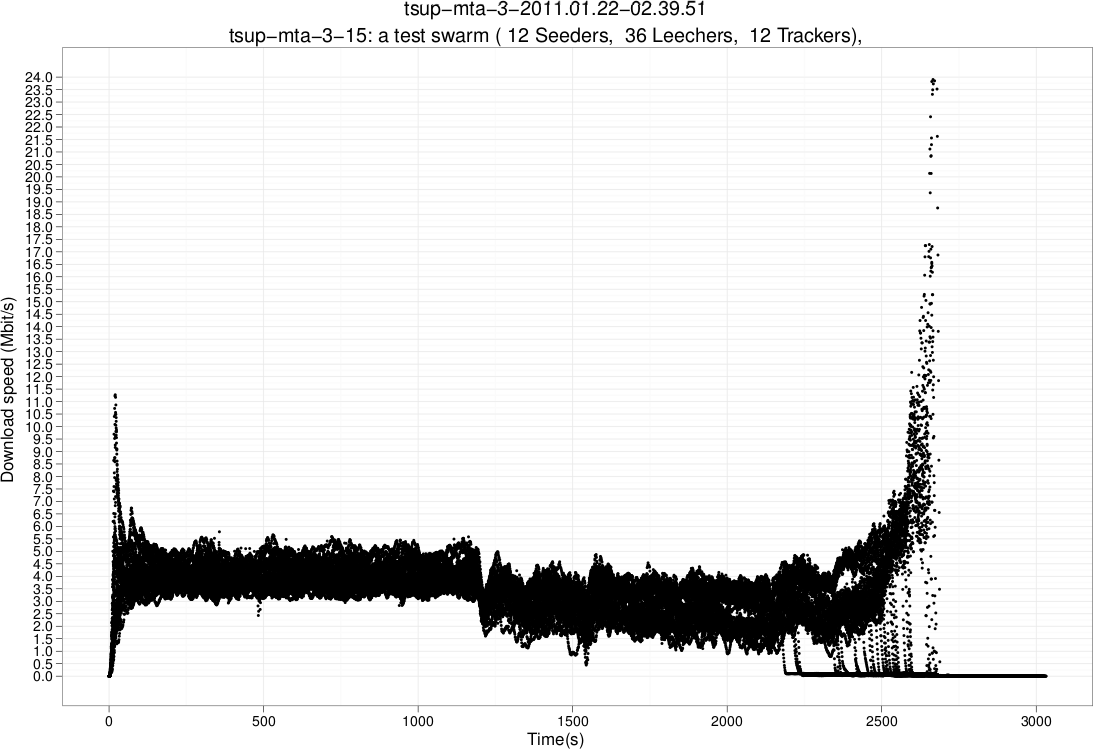
\includegraphics[width=0.7\textwidth]{src/img/unified-tracker/tsup-sample-run-48peers}
  \end{center}
  \caption{Sample Run Graphic}
  \label{fig:unified-tracker:tsup-sample-run}
\end{figure}

An automatically-generated sample output graphic, describing a 48 peer session
(12 seeders, 36 leechers, 12 trackers) sharing a 1024 MB file is shown in
Figure~\ref{fig:unified-tracker:tsup-sample-run}. The image presents download
speed evolution for all swarm peers. All of them are limited to 24 Mbit
download speed and 3 Mbit upload speed.

All peers use download speed between 2 Mbit and 5 Mbit on the first 2000
seconds of the swarm's lifetime. As the leechers become seeders, the swarm
download speed increases rapidly as seen in the last part of the swarm's
lifetime, with the last leechers reaching the top speed of 24 Mbit.

\section{Experimental Results and Evaluation}
\label{sec:unified-tracker:results}

In order to test the overhead added by TSUP to BitTorrent protocol, we have
made a set of test scenarios which compare the average download speed for a
swarm with unified trackers and for another swarm with just one non-unified
tracker, but the same number of leechers and seeders. Each test scenario is
characterized by the shared file sizes, the number of peers and, in the case
of tests with unified trackers, by the number of trackers. We shared 3 files
of sizes 64MB, 256MB and 1024MB.

In the test scenarios with unified trackers for each file we tested the swarm
with 1, 2, 4, 8 and 12 trackers. On each tracker there were connected 4 peers,
from which 1 is a seeder and 3 are leechers. So, for example, in a scenario
with 8 trackers there are 8 seeders and 24 leechers, totalizing 32 peers.
Having 3 files and 12 trackers in the biggest scenario we needed to create 36
.torrent files, because for each shared file we made a .torrent file for each
tracker. In the corresponding test scenarios with non-unified trackers, there
is just one .torrent file for each shared file. We varied the numbers of
seeders and leechers connected to the tracker so that they have the same
cardinality with the corresponding unified trackers scenarios.

Each test scenario has been repeated \textit{20 times} in order to allow
statistical relevance. The average download speed was calculated as an average
value from the 20 sessions.

Results may be seen in Table~\ref{tab:unified-tracker:comparison}, which
depicts the results for each file size, in the top (64MB), middle (256MB) and
bottom part of it (1024MB), respectively. For each of this two situations the
mean download speed (``mean dspeed'') and relative standard deviation
(``rel.st.dev.'') is depicted. In the right part, titled ``perf. Decrease''
(performance decrease), shows the percent of download speed decrease induced
by the overhead of the TSUP. In the left side of the table the number of
seeders and leechers for each scenario is shown. The percentage value for
download speed decrease is computed using the standard formula:

%\vspace{3mm}

\begin{equation}\label{updates-swarmleader}
d = 100\% \cdot \frac{ds_{SingleTracker} - ds_{UnifiedTrackers}}{ds_{SingleTracker}} ,
\end{equation}

%\vspace{2mm}

where \textit{ds} is an abbreviation from mean download speed.

%\vspace{3mm}

All positive percentage values from the ``perf. decrease'' header mark a
decrease of performance caused by TSUP overhead. A negative download speed
decrease percentage shows that there is an increase instead of a decrease.

The unification which takes place in XBT Unified Tracker introduces an
overhead in the BitTorrent protocol in comparison to XBT Tracker. In theory
the performance decrease must always be positive. But there are situations
where percentages are negative, which could suggest that TSUP increases
the speed, thus reducing the download time. But this performance increase is
not due to TSUP, but is caused by another fact. In all scenarios, in the
Single Tracker experiments, at the beginning, all peers are started almost
simultaneously, creating a flash crowd. In this situation, communication
between peers will start immediately, but when multiple trackers are unified,
the TSUP imposes a delay before each peer finds out of all the others, because
of the convergence time.  It is known that sometimes it is better when peers
enter the swarm later~\cite{bt-analysis}, explaining the presence of negative
values for the performance decrease.

%\begin{figure}[h]
%  \begin{center}
%    \includegraphics[width=\columnwidth]{src/img/unified-tracker/table-results.png}
%  \end{center}
%  \caption{Tracker Networks}
%  \label{fig:unified-tracker:table-results}
%\end{figure}

\def \singlesods {337.73}
\def \singlestds {472.27}
\def \singlesfds {475.13}
\def \singleseds {476.10}
\def \singleswds {470.53}
\def \singlesorsd {1.28}
\def \singlestrsd {0.87}
\def \singlesfrsd {1.87}
\def \singlesersd {6.06}
\def \singleswrsd {9.61}

\def \singletods {358.72}
\def \singlettds {476.59}
\def \singletfds {477.56}
\def \singleteds {492.40}
\def \singletwds {486.04}
\def \singletorsd {0.45}
\def \singlettrsd {0.26}
\def \singletfrsd {0.45}
\def \singletersd {6.64}
\def \singletwrsd {8.33}

\def \singleoods {365.27}
\def \singleotds {477.47}
\def \singleofds {477.54}
\def \singleoeds {423.71}
\def \singleowds {407.71}
\def \singleoorsd {0.19}
\def \singleotrsd {0.15}
\def \singleofrsd {0.18}
\def \singleoersd {6.19}
\def \singleowrsd {4.47}

\def \multiplesods {335.11}
\def \multiplestds {396.55}
\def \multiplesfds {463.42}
\def \multipleseds {497.35}
\def \multipleswds {496.48}
\def \multiplesorsd {2.87}
\def \multiplestrsd {16.64}
\def \multiplesfrsd {12.60}
\def \multiplesersd {11.10}
\def \multipleswrsd {11.48}

\def \multipletods {356.55}
\def \multiplettds {407.55}
\def \multipletfds {477.45}
\def \multipleteds {500.56}
\def \multipletwds {494.93}
\def \multipletorsd {1.07}
\def \multiplettrsd {14.67}
\def \multipletfrsd {10.73}
\def \multipletersd {8.49}
\def \multipletwrsd {12.38}

\def \multipleoods {365.57}
\def \multipleotds {437.09}
\def \multipleofds {466.03}
\def \multipleoeds {418.69}
\def \multipleowds {418.76}
\def \multipleoorsd {0.31}
\def \multipleotrsd {9.12}
\def \multipleofrsd {5.93}
\def \multipleoersd {8.73}
\def \multipleowrsd {6.27}


\begin{sidewaystable}
  \centering
  \caption{Single Tracker vs. Unified Trackers Comparison}
  \label{tab:unified-tracker:comparison}
  \begin{tabular}{@{}rrcccrccc@{}}
    \toprule
       & & \multicolumn{2}{c}{\textbf{Single Tracker}} & &
       \multicolumn{3}{c}{\textbf{Unified
       Trackers}} & \\
    \cmidrule{3-4} \cmidrule{6-8}
      \textit{seeders} & \textit{leechers} & \textit{mean dspeed (KB/s)} &
      \textit{rel.st.dev. (\%)} & & \textit{trackers} & \textit{mean dspeed (KB/s)} &
      \textit{rel.st.dev. (\%)} & \textit{perf. decrease (\%)} \\
    \midrule
      $size = 64MB$\\
      1 & 3 & \singlesods & \singlesorsd & & 1 & \multiplesods &
      \multiplesorsd & 0.78 \\  %01
      2 & 6 & \singlestds & \singlestrsd & & 6 & \multiplestds &
      \multiplestrsd & 16.03 \\  %04
      4 & 12 & \singlesfds & \singlesfrsd & & 4 & \multiplesfds &
      \multiplesfrsd & 2.46 \\  %07
      8 & 24 & \singleseds & \singlesersd & & 8 & \multipleseds &
      \multiplesersd & -4.46 \\  %10
      12 & 36 & \singleswds & \singleswrsd & & 12 & \multipleswds &
      \multipleswrsd & -5.52 \\ %13
      $size = 256MB$\\
      1 & 3 & \singletods & \singletorsd & & 1 & \multipletods &
      \multipletorsd & 0.6 \\   %02
      2 & 6 & \singlettds & \singlettrsd & & 6 & \multiplettds &
      \multiplettrsd & 14.49 \\   %05
      4 & 12 & \singletfds & \singletfrsd & & 4 & \multipletfds &
      \multipletfrsd & 0.02 \\  %08
      8 & 24 & \singleteds & \singletersd & & 8 & \multipleteds &
      \multipletersd & -1.66 \\  %11
      12 & 36 & \singletwds & \singletwrsd & & 12 & \multipletwds &
      \multipletwrsd & -1.83 \\ %14
      $size = 1024MB$\\
      1 & 3 & \singleoods & \singleoorsd & & 1 & \multipleoods &
      \multipleoorsd & -0.08 \\   %03
      2 & 6 & \singleotds & \singleotrsd & & 6 & \multipleotds &
      \multipleotrsd & 8.46 \\   %06
      4 & 12 & \singleofds & \singleofrsd & & 4 & \multipleofds &
      \multipleofrsd & 2.41 \\  %09
      8 & 24 & \singleoeds & \singleoersd & & 8 & \multipleoeds &
      \multipleoersd & 1.18 \\  %12
      12 & 36 & \singleowds & \singleowrsd & & 12 & \multipleowds &
      \multipleowrsd & -2.71 \\ %15
    \bottomrule
  \end{tabular}
\end{sidewaystable}


From results in Table~\ref{tab:unified-tracker:comparison} several
conclusions are drawn.  The TSUP overhead decreases, on the
first hand, when the number of peers increases (and proportionally the number
of seeders) and, on the other hand, when the file size increases. When the
overhead is insignificant, the percentages have lower values. TSUP convergence
time causes the avoidance of a flash crown at the beginning of each scenario,
thus inducing a small performance increase. Starting from 8 seeders and more
TSUP performance decrease becomes smaller than the performance increase caused
by avoiding the flash crowd. That is why some performance decrease values are
negative. The relative standard deviation is generally increasing with the
number of peers, but is decreasing when the file size increases. The values
can be considered normal, taking into account the number of peers that are
part of a swarm.

Swarm unification increases the number of peers for a shared file, but this
fact does not always grant a larger download speed, as it can be seen in
Table~\ref{tab:unified-tracker:comparison}. However, having a swarm with a
bigger number of peers has three advantages. First of all, it increases the chance
that more seeders will later be available and a big proportion of stable
seeders increase download speed. The second reason is that bigger swarms
increase a shared file's availability by creating redundancy. The third reason
is
that a bigger swarm is more attractive for new users, giving the possibility
of creating a big network which may be used for features such as social
networking.
